% Chapter 2: The breadth-first walk
% Contains:
%   The definition of the breadth-first walk
%   The continuous version
%   The proof of Zn -> W

\chapter{The breadth-first walk} \label{C: bf-walk}
\fxnote{Update title.}


\section{The discrete breadth-first walk}
%%%%%%%%%%%%%%%%%%%%%%%%%%%%%%%%%%%%%%%%%%%%%%%%%%%%%%%%%%%%
% SECTION: The discrete breadth-first walk
%%%%%%%%%%%%%%%%%%%%%%%%%%%%%%%%%%%%%%%%%%%%%%%%%%%%%%%%%%%%
\fxnote{Update title}

%%%%%%%%%%%%%%%%%%%%%%%%%%%%%%%%%%%%%%%%%%%%%%%%%%%%%%%%%%%%
% Introduction
%%%%%%%%%%%%%%%%%%%%%%%%%%%%%%%%%%%%%%%%%%%%%%%%%%%%%%%%%%%%
We start by describing the deterministic construction of the breadth-first walk.
\fxnote{More free from paper}
Consider an arbitrary graph $\mathcal{G}$ on the set of vertices 
$\{1, \dots , n\} $.
We will define the breadth-first ordering
$(v(1), \dots v(n))$
of the vertices along with an integer-valued sequence
$(z(i), \; 1 \leq i \leq n)$
which we call the breadth-first walk on
$\mathcal{G}$.


%%%%%%%%%%%%%%%%%%%%%%%%%%%%%%%%%%%%%%%%%%%%%%%%%%%%%%%%%%%%
% Definition of breadth-first order
%%%%%%%%%%%%%%%%%%%%%%%%%%%%%%%%%%%%%%%%%%%%%%%%%%%%%%%%%%%%
The breadth-first order follow an algorithmic construction as follows:
Let $\Ci{1}, \Ci{2}, \dots$ be the components of $\mathcal{G}$ in order, such that
$w_1, w_2, \dots$, the vertices with the smallest label in the corresponding component,
are ordered $w_1 > w_2 > \dots$. 
Call $w_i$ the root of $\Ci{i}$.
Now order by levels (distance from the root) and within levels order by original vertex label.
See Figure~\ref{F: bf-walk discrete} for an example of the new ordering.

For a more mathematically concise definition,
consider the set of vertices $\{ v(1),\dots, v(i) \}$
and define the \emph{neighbour set} $\Ni{i}$ as the vertices outside of
\fxnote{Add emphasis when needed}
$\{ v(1),\dots, v(i) \}$ 
that are neighbours to some vertex in 
$\{ v(1),\dots, v(i) \}$:
\begin{equation}
\Ni{i} := 
\left\lbrace v \in \{1, \dots, n\} \backslash \{ v(1),\dots, v(i) \} 
\; | \; 
\left(v(j), v\right) \in S \; \text{for some} \; 1 \leq j \leq i \right\rbrace
\end{equation}
\fxnote{Remove equation? Unnecessary?}
\fxnote{Fix \text in braces: Space \; or \quad}
This allows us to define the set of children of some vertex $v(i)$ as
$\Ni{i} \backslash \Ni{i-1}$.
First order the components as described above. 
Now consider only the first component $\Ci{1}$.
Define $v(1) := w_1$, the root of $\Ci{1}$ and define
$v(2), \dots , v(1 + |\Ni{1}|)$ 
as the neighbours of $v(1)$,
in increasing order of vertex label. 
Define the new label for all 
$i = 2, \dots, |\Ci{1}|$,
that is all vertices in the first component,
inductively by listing all children (if any exist) of $v(i)$
in increasing order as 
$ v(i + |\Ni{i-1}|), \dots, v(i + |\Ni{i}|) $.
After labeling the last vertex in $\Ci{1}$, set
$v(|\Ci{1}| + 1) := w_2$, 
the root of $\Ci{2}$, and continue the construction as above.
Traverse all components this way.


%%%%%%%%%%%%%%%%%%%%%%%%%%%%%%%%%%%%%%%%%%%%%%%%%%%%%%%%%%%%
% Definitions of breadth-first walk
%%%%%%%%%%%%%%%%%%%%%%%%%%%%%%%%%%%%%%%%%%%%%%%%%%%%%%%%%%%%
For the number of children of $v(i)$ write 
$c(i) = |\Ni{i} \backslash\Ni{i-1}|$.
Now define the breadth-first walk 
$(z(i), \; 1 \leq i \leq n)$
by
\begin{equation} \label{E: def bf-walk z}
\begin{aligned}
z(0) &:= 0, \\
z(i) &:= z(i-1) + c(i) -1, \quad i=1, \dots , n.
\end{aligned}
\end{equation}


%%%%%%%%%%%%%%%%%%%%%%%%%%%%%%%%%%%%%%%%%%%%%%%%%%%%%%%%%%%%
% Explanation
%%%%%%%%%%%%%%%%%%%%%%%%%%%%%%%%%%%%%%%%%%%%%%%%%%%%%%%%%%%%
An explanation:
\fxnote{Change this}
The process divides the vertex-set into three parts: 
Explored, discovered and neutral vertices. Every vertex starts as neutral.
At step $1$, we traverse vertex $v(1)$ and mark it as explored.
We search for neighbours of $v(1)$, and mark these as discovered.
The next vertex to explore is the vertex already discovered with the smallest label,
and each vertex switches from neutral to discovered once it gets assigned a new label.
Once it's neighbours are explored, it switches to explored.
\fxnote{This whole paragraph}
Note that after traversing every vertex of one component, 
there are no discovered vertices left.
The walk $z$ decreases by $1$ for each vertex traversed
and increases by the number of new neighbours explored in each step.


\begin{figure}[H]
	
	\centering
	\subfloat[Original vertex labels]
	{\begin{tikzpicture}[level distance = 11mm, scale = 1]
	\tikzstyle{level 1}=[sibling distance=8mm]
	\tikzstyle{level 2}=[sibling distance=8mm]
	\tikzstyle{level 3}=[sibling distance=8mm]
	
	\node [plain] (1) {1} [grow=up]
	child { node [plain] {\phantom{0}}
		child { node [plain] {\phantom{0}}
		}
		child { node [plain] {\phantom{0}}
		}
	}
	child { node [plain] {\phantom{0}}
	}
	;
	\node [plain] [right=2.5cm of 1] (6) {2} [grow=up]
	child { node [plain] {\phantom{0}}
		child { node [plain] {6}
		}
		child { node [plain] {\phantom{0}}
		}
		child { node [plain] {\phantom{0}}
		}
	}
	child { node [plain] (8) {\phantom{0}}
	}
	child { node [plain] {\phantom{0}}
		child { node [plain] (10) {\phantom{0}}
		}
	}
	;
	\node [plain] [right=2cm of 6] (14) {3} [grow=up]
	child { node [plain] {\phantom{0}}
	}
	;
	\node [plain] [right=1cm of 14] (16) {4} [grow=up]
	child { node [plain] {\phantom{0}}
	}
	child { node [plain] {\phantom{0}}
	}
	;
	\node [plain] [right=1cm of 16] (19) {5}
	;
	\node [plain] [right=1cm of 19] (20) {7} [grow=up]
	child { node [plain] {\phantom{0}}
	}
	child { node [plain] {\phantom{0}}
		child { node [plain] {\phantom{0}}
			child { node [plain] {\phantom{0}}
			}
			child { node [plain] {\phantom{0}}
			}
			child { node [plain] {\phantom{0}}
			}
			child { node [plain] {\phantom{0}}
			}
		}
	}
	;
	\draw (10) -- (8);
\end{tikzpicture}}\\
	
	\centering
	\subfloat[New vertex labels]
	{\begin{tikzpicture}[level distance = 11mm, scale = 1]
	\tikzstyle{level 1}=[sibling distance=8mm]
	\tikzstyle{level 2}=[sibling distance=8mm]
	\tikzstyle{level 3}=[sibling distance=8mm]
	
	\node [plain] (1) {1} [grow=up]
	child { node [plain] {3}
		child { node [plain] {5}
		}
		child { node [plain] {4}
		}
	}
	child { node [plain] {2}
	}
	;
	\node [plain] [right=2.5cm of 1] (6) {6} [grow=up]
	child { node [plain] {9}
		child { node [plain] {13}
		}
		child { node [plain] {12}
		}
		child { node [plain] {11}
		}
	}
	child { node [plain] (8) {8}
	}
	child { node [plain] {7}
		child { node [plain] (10) {10}
		}
	}
	;
	\node [plain] [right=2cm of 6] (14) {14} [grow=up]
	child { node [plain] {15}
	}
	;
	\node [plain] [right=1cm of 14] (16) {16} [grow=up]
	child { node [plain] {18}
	}
	child { node [plain] {17}
	}
	;
	\node [plain] [right=1cm of 16] (19) {19}
	;
	\node [plain] [right=1cm of 19] (20) {20} [grow=up]
	child { node [plain] {22}
	}
	child { node [plain] {21}
		child { node [plain] {23}
			child { node [plain] {27}
			}
			child { node [plain] {26}
			}
			child { node [plain] {25}
			}
			child { node [plain] {24}
			}
		}
	}
	;
	\draw (10) -- (8);
\end{tikzpicture}}\\
	
	\centering
	\subfloat[Resulting breadth-first walk, dashed lines indicating the end of components]
	{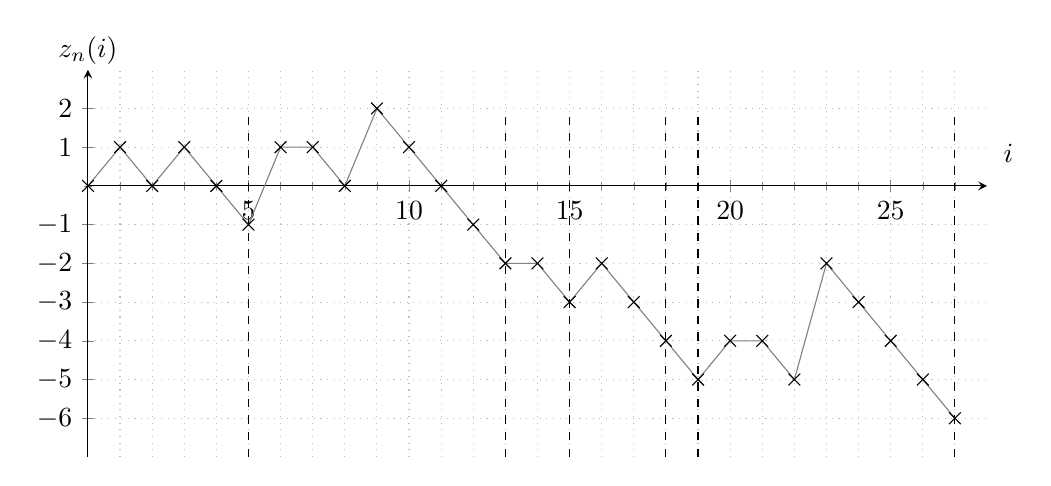
\begin{tikzpicture}

\begin{axis}[
axis x line=bottom,
axis y line=left,
grid = minor,
minor grid style={dotted},
xmin=0,
axis lines = middle,
xmax=28,
ymax = 3,
ymin  = -7,
xlabel={$i$},
x label style = {at={(axis description cs:1.04,0.785)},anchor=east},
ylabel={$z_n(i)$},
y label style = {at={(axis description cs:0,1.11)},anchor=north},
xtick={5,10,15,20,25},
minor xtick = {1,...,27},
ytick={-6,...,2},
minor ytick={-6,...,2},
width = 13cm,
height = 6.5cm
]

\addplot [
mark=x,
mark options={color=black, scale=1.5}, 
color=gray
]
coordinates{
	(0,0) (1,1) (2,0) (3,1) (4,0) (5,-1)
	(6,1) (7,1) (8,0) (9,2) (10,1) (11,0) (12,-1) (13,-2) 
	(14,-2) (15,-3) 
	(16,-2) (17,-3) (18,-4) 
	(19,-5) 
	(20, -4) (21,-4) (22,-5) (23,-2) (24,-3) (25,-4) (26, -5) (27,-6)
};


\addplot [dashed] coordinates {(5, -7) (5, 2)};
\addplot [dashed] coordinates {(13, -7) (13, 2)};
\addplot [dashed] coordinates {(15, -7) (15, 2)};
\addplot [dashed] coordinates {(18, -7) (18, 2)};
\addplot [dashed] coordinates {(19, -7) (19, 2)};
\addplot [dashed] coordinates {(27, -7) (27, 2)};
\end{axis}

\end{tikzpicture} }
	
	\caption{Breadth-first walk on the first components of a graph}
	\label{F: bf-walk discrete}
\end{figure} 
\fxnote{Fix centering of figure captions}
\fxnote{Add more vertex labels in original ordering?}


%%%%%%%%%%%%%%%%%%%%%%%%%%%%%%%%%%%%%%%%%%%%%%%%%%%%%%%%%%%%
% Equivalent definition
%%%%%%%%%%%%%%%%%%%%%%%%%%%%%%%%%%%%%%%%%%%%%%%%%%%%%%%%%%%%
We write
\begin{align}
\zeta(j) &:= |\Ci{1}| + \dots + |\Ci{j}|, \label{E: zeta}\\ 
\ZetaMinus{i} &:= \min \{ j \; | \; \zeta(j) \geq i \}, \label{E: zeta-1}
\end{align}
for the index of the last vertex in the $j$-th component (that's \eqref{E: zeta})
and \eqref{E: zeta-1}, the index of the component containing $v(i)$.
\fxnote{This sentence is a test for labeling of align-equs. Fix!}
Now we can provide a definition of the breadth-first walk equivalent to \eqref{E: def bf-walk z}:
\begin{equation}  \label{E: def bf-walk z*}
\begin{aligned}
z^*(0) &:= 0, \\
z^*(i) &:= |\Ni{i}| - \zeta^{-1}(i), \quad i=1, \dots , n.
\end{aligned}
\end{equation}

We verify the equivalence by induction.
We show that, for $i \geq 2$, increments of both functions are equal,
so
\begin{equation} \label{E: equality z z*}
\begin{aligned} 
&\hspace{35pt} z(i) - z(i-1) = z^*(i)  -z^*(i-1) \\
&\iff c(i) - 1 = |\Ni{i}| - \ZetaMinus{i} - |\Ni{i-1}| + \ZetaMinus{i-1} \\
&\iff |\Ni{i}| - |\Ni{i-1}| = c(i) + \ZetaMinus{i} - \ZetaMinus{i-1}
\end{aligned}
\end{equation}
\fxnote{This equation does not look nice. Delete 1./2. row? Delete iffs?}
\fxnote{This has to hold for i >= 1, or fix the indices.}

We divide the proof into two cases.
First, assume $v(i-1)$ is not the last vertex in it's component.
Then $v(i)$ belongs to the same component and
$\ZetaMinus{i} = \ZetaMinus{i-1}$.
Vertex $v(i)$ has already been assigned a new label at step $i-1$,
so $v(i) \in \Ni{i-1}$.
Going from $i-1$ to $i$,
$\Ni{*}$ increases by the number of new neighbours of $v(i)$
and decreases by $v(i)$ itself.
So
\begin{equation}
|\Ni{i}| - |\Ni{i-1}| = c(i) - 1,
\end{equation}
which proves the equivalence.

In the second case, if $v(i-1)$ is the last vertex of it's component,
then $\ZetaMinus{i} = \ZetaMinus{i-1} + 1$
and $|\Ni{i-1}| = 0$.
Equality \eqref{E: equality z z*} reduces to
$ |\Ni{i}| = c(i)$,
which holds since
$c(i) = |\Ni{i} \backslash \Ni{i-1}| = |\Ni{i}|$.

Since $|\Ni{i}| = 0$ only if $v(i)$ is the last vertex in its component,
\fxnote{Have we shown this? Maybe add a sentence.}
\fxnote{its or it's? Fix in whole document!}
\eqref{E: zeta} and \eqref{E: def bf-walk z*} imply
\begin{equation}
	z(\zeta (j)) = -j
\end{equation}
and 
\begin{equation}
	z(i) \geq -j \quad \text{for all} \enspace \zeta(j) < i < \zeta(j+1).
\end{equation}

So, for vertices in the $j$-th component,
the random walk takes values greater or equal to $-(j-1)$,
until the last vertex, for which $z$ reaches a new minimum at $-j$.
\fxnote{There are a lot of commas in this sentence.}
Knowing this we can reconstruct sizes and indices of components via
\begin{align}
\zeta(j) &= \min \{ i \; | \; z(i) = -j \}, \label{E: zeta(j) = min(i)} \\
|\Ci{j}| &= \zeta(j) - \zeta(j-1), \label{E: C(j) = zeta - zeta} \\
\ZetaMinus{i} &= 1 - \min_{j \leq i-1}z(j). \label{E: zeta-1(i) = 1 - min(j)}
\end{align}
\fxnote{Maybe add some more explanation on where these formulas come from.}

\fxnote{Transition to next chapter here.}

\section{The continuous breadth-first walk}
%%%%%%%%%%%%%%%%%%%%%%%%%%%%%%%%%%%%%%%%%%%%%%%%%%%%%%%%%%%%
% SECTION: The continuous breadth-first walk
%%%%%%%%%%%%%%%%%%%%%%%%%%%%%%%%%%%%%%%%%%%%%%%%%%%%%%%%%%%%

The last section defined the random walk for integer times,
but to develop our theory of convergence to a Brownian motion
we will have to construct $z(i)$ in continuous time.

Define a series of independent random variables, 
uniformly distributed on $(0,1)$, 
$(\Uij, 1 \leq i \leq n, 1 \leq j \leq c(i))$.
\fxnote{Series is probably a bad term, since it's already a math term.}

Then for each $i = 1, 2, \dots$ and $0 \leq u \leq 1$ define the process $Z$ by
\begin{equation} \label{E: def Z}
\begin{aligned}
Z(0) &:= 0, \\
Z(i - 1 + u) &:= Z(i-1) - u + \sum_{1 \leq j \leq c(i)} \Ind{\{ \Uij \leq u \}}.
\end{aligned}
\end{equation}
\fxfatal{Find the other indicator function and use the same method there.}
So $Z(i) = Z(i-1) - 1 + c(i)$ 
and $Z$ coincides with the discrete definition of the breadth-first walk at integer times.

Some more explanation on this construction:
\fxnote{Start this paragraph nicer.}
At time $i-1$, 
the walk has traversed vertices
$(v(1), \dots, v(i-1))$
and has encountered a list of vertices
$(v(1), \dots, v(k))$
of length
$k = i-1 + |\Ni{i-1}|$.
The discrete walk now adds the children of $v(i)$,
$c(i)$, to this list at time $i$.
The newly defined continuous walk adds those vertices at uniformly random times in $(i-1, i)$.

\begin{figure}[H]
	\centering
	\subfloat[A graph component]
	{\begin{tikzpicture}[level distance = 11mm, scale = 1]
	\tikzstyle{level 1}=[sibling distance=8mm]
	\tikzstyle{level 2}=[sibling distance=8mm]
	\tikzstyle{level 3}=[sibling distance=8mm]
	
	\node [plain] [right=2.5cm of 1] (1) {1} [grow=up]
	child { node [plain] {4}
		child { node [plain] {8}
		}
		child { node [plain] {7}
		}
		child { node [plain] {6}
		}
	}
	child { node [plain] (3) {3}
	}
	child { node [plain] {2}
		child { node [plain] (5) {5}
		}
	}
	;
\end{tikzpicture}}\\
	
	\centering
	\subfloat[The continuous breadth-first walk]
	{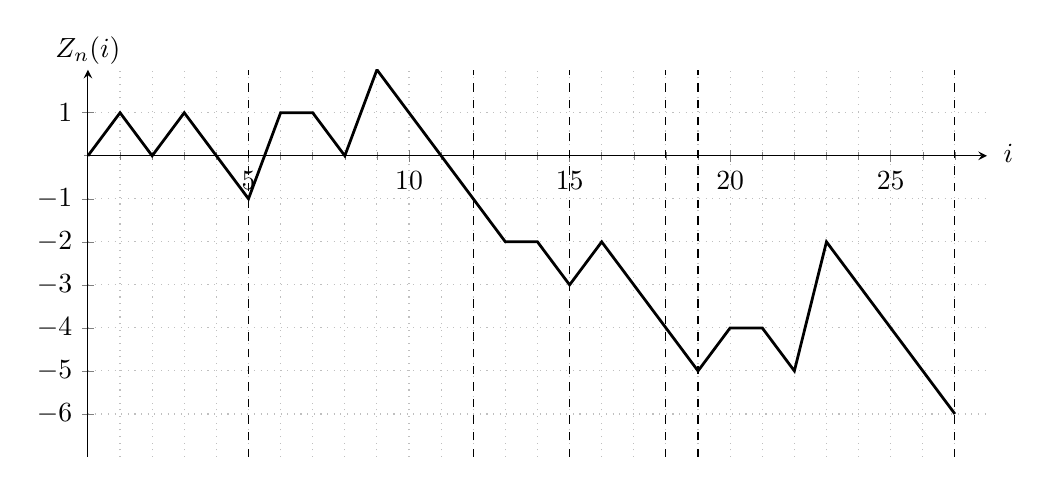
\begin{tikzpicture}

\begin{axis}[
axis x line=bottom,
axis y line=left,
grid = minor,
minor grid style={dotted},
xmin=0,
axis lines = middle,
xmax=28,
ymax = 2,
ymin  = -7,
xlabel={$i$},
x label style = {at={(axis description cs:1.04,0.785)},anchor=east},
ylabel={$Z_n(i)$},
y label style = {at={(axis description cs:0,1.11)},anchor=north},
xtick={5,10,15,20,25},
minor xtick = {1,...,27},
ytick={-6,...,1},
minor ytick={-6,...,1},
width = 13cm,
height = 6.5cm
]

\addplot [
line width=1.0pt
]
coordinates{
	(0,0) (1,1) (2,0) (3,1) (4,0) (5,-1)
	(6,1) (7,1) (8,0) (9,2) (10,1) (11,0) (12,-1) (13,-2) 
	(14,-2) (15,-3) 
	(16,-2) (17,-3) (18,-4) 
	(19,-5) 
	(20, -4) (21,-4) (22,-5) (23,-2) (24,-3) (25,-4) (26, -5) (27,-6)
};

\addplot [dashed] coordinates {(5, -7) (5, 2)};
\addplot [dashed] coordinates {(12, -7) (12, 2)};
\addplot [dashed] coordinates {(15, -7) (15, 2)};
\addplot [dashed] coordinates {(18, -7) (18, 2)};
\addplot [dashed] coordinates {(19, -7) (19, 2)};
\addplot [dashed] coordinates {(27, -7) (27, 2)};
\end{axis}

\end{tikzpicture} }
	
	\caption{Continuous breadth-first walk on a single component}
	\label{F: bf-walk cont}
\end{figure} 
\fxfatal{Here comes a figure and some illustration.}


For $\mathcal{G} \in \Gnt$, 
we call the continuous breadth-first walk on its vertices $Z_n^t$.
We rescale $Z_n^t$ on both axis to define
\begin{equation} \label{E: def Zbar}
\bar{Z}^t_n(s) := \n{-1}{3} Z_n^t(\n{2}{3}s).
\end{equation}
For $s \geq \n{1}{3}$, 
let $Z_n^t(\n{2}{3}s) \equiv Z_n^t(n)$.
\fxnote{Is equiv right here? Or just use :=?}
We can now state the main theorem of this chapter,
the convergence of this rescaled process to a Brownian motion.

\begin{theorem} \label{T: Z -> W}
	Let $Z_n^t(s)$, for $0 \leq s \leq n$, 
	be the breadth-first walk associated with $\mathcal{G} \in \Gnt$.
	Rescale via
	\begin{equation*}
	\bar{Z}^t_n(s) := \n{-1}{3} Z_n^t(\n{2}{3}s).
	\end{equation*}
	Then $\bar{Z}^t_n(s) \rightarrow_d \Wt$ as $n \rightarrow \infty$.
\end{theorem}

\fxfatal{A short explanantion of the coming proof goes here.}


\section{Decompositions of $Z_n$}
%%%%%%%%%%%%%%%%%%%%%%%%%%%%%%%%%%%%%%%%%%%%%%%%%%%%%%%%%%%%
% SECTION: Decompositions of $Z_n$
%%%%%%%%%%%%%%%%%%%%%%%%%%%%%%%%%%%%%%%%%%%%%%%%%%%%%%%%%%%%
\fxfatal{Update title}
\fxnote{is splitting the proof into 3 sections necessary?}
\fxnote{Add introductory text}

For ease of notation, we will drop the superscript $t$ from all random variables.


%%%%%%%%%%%%%%%%%%%%%%%%%%%%%%%%%%%%%%%%%%%%%%%%%%%%%%%%%%%%
% Lemma Decompositions An: Statement
%%%%%%%%%%%%%%%%%%%%%%%%%%%%%%%%%%%%%%%%%%%%%%%%%%%%%%%%%%%%
\begin{lemma} \label{L: decomp Zn}
	The decomposition 
	\begin{equation} \label{E: decomp Zn}
	Z_n = M_n + A_n
	\end{equation}
	holds, where $M_n$ is a martingale and $A_n$ is defined by
	\begin{equation} \label{D: An}
	\An{t} = \int_{0}^{t} a_n(s)ds - t
	\end{equation}
	with
	\begin{equation} \label{D: an}
	a_n(s)ds = \Prob(\text{A new edge appears in} \enspace [s, s+ds] \cond \Zn{u}, \enspace u \leq s).
	\end{equation}	
	\fxnote{Make text in P() not cursive?}
\end{lemma}

%%%%%%%%%%%%%%%%%%%%%%%%%%%%%%%%%%%%%%%%%%%%%%%%%%%%%%%%%%%%
% Lemma Decompositions An: Proof
%%%%%%%%%%%%%%%%%%%%%%%%%%%%%%%%%%%%%%%%%%%%%%%%%%%%%%%%%%%%
\begin{proof} \label{P: decomp Zn}
	We will prove that $Z_n - A_n$ is a martingale by showing that
	\begin{equation} \label{E: Mn martingale}
	\Exp{ \Zn{t+u} - \An{t+u} \cond \F{t} } = \Zn{t} - \An{t}
	\end{equation}
	holds for all $u \geq 0$, where $\F{t}$ is the natural $\sigma$-algebra generated by $Z_n$, 
	$\F{t} = \sigma(\Zn{s}, s \leq t).$
	This is equivalent to 
	\begin{equation}
	\Exp{\Zn{t+u} - \Zn{t} \cond \F{t}} = \Exp{\An{t+u} - \An{t} \cond \F{t}}.
	\end{equation}
	
	We start with the left-hand side. 
	The change of $Z_n$ between times $t$ and $t+u$ is the sum of all jumps that occurred in $[t, t+u]$,
	minus the constant downward drift $u$:
	\begin{align*}
	\Exp{\Zn{t+u} - \Zn{t} \cond \F{t}} 
	&= \Exp{\text{Number of jumps in} \enspace [t, t+u] \cond \F{t}} - u \\
	&= \Exp{\text{Number of new edges appearing in} \enspace [t, t+u] \cond \F{t}} - u,
	\end{align*}
	since every new edge corresponds to a jump of size $1$ in $Z_n$.
	
	Looking at the right-hand side, we define $\NewEdge{I}$ as the event of a new edge appearing during the time interval $I$ and calculate
	\begin{align*}
	\Exp{\An{t+u} - \An{t} \cond \F{t}}
	&= \Exp{ \int_{0}^{t+u} a_n(s)ds - (t+u) - \int_{0}^{t} a_n(s)ds + t \cond \F{t} } \\
	&= \Exp{ \int_{t}^{t+u} a_n(s)ds \cond \F{t} } - u \\
	&= \int_{t}^{t+u} \Exp{a_n(s)ds \cond \F{t}} - u \\
	&= \int_{t}^{t+u} \Exp{ \Prob(\NewEdge{\sds} \cond \F{s}) \cond \F{t} } - u\\
	&= \int_{t}^{t+u} \Prob( \NewEdge{\sds} \cond \F{t} ) - u
	\quad \text{since} \enspace \F{s} \subseteq \F{t} \enspace \forall s \in [t,t+u] \\
	&= \Exp{\text{Number of new edges appearing in} \enspace [t, t+u] \cond \F{t}} - u.
	\end{align*}
	\fxnote{Fs in Ft or Ft in Fs? Use "tower property".}
	\fxnote{Explain "Number of new edges"="int P" more detailed.}
	
	This proves $M_n$ to be a martingale. 	
\end{proof}


%%%%%%%%%%%%%%%%%%%%%%%%%%%%%%%%%%%%%%%%%%%%%%%%%%%%%%%%%%%%
% Lemma Formula An: Statement
%%%%%%%%%%%%%%%%%%%%%%%%%%%%%%%%%%%%%%%%%%%%%%%%%%%%%%%%%%%%
\begin{lemma} \label{L: formula an}
	For $a_n$ as defined in Lemma~\ref{L: decomp Zn},
	\begin{equation}
	\an{s} = (n - s - \Zetan{\ceil{s}} - \Zn{s}) \ps .
	\end{equation}
	\fxnote{Update/change Zeta-symbol if needed.}
	\fxnote{Add explanation of Zeta if needed.}
\end{lemma}

%%%%%%%%%%%%%%%%%%%%%%%%%%%%%%%%%%%%%%%%%%%%%%%%%%%%%%%%%%%%
% Lemma Formula An: Proof
%%%%%%%%%%%%%%%%%%%%%%%%%%%%%%%%%%%%%%%%%%%%%%%%%%%%%%%%%%%%
\begin{proof} \label{P: formula an}
	Consider the walk $Z_n$ at time $s\in[i-1, i]$.
	Let $N$ be the number of vertices that, at time $i-1$, were eligible to be children of vertex $v(i)$.
	That is, all vertices not yet explored or discovered, and excluding $v(i)$ itself.
	To any eligible vertex $j$ we assign a random variable $\Uij$.
	Let all $\Uij$ be independent and identically $\mathcal{U}(0,1)$ distributed.
	Our understanding of the process of discovering children of $v(i)$ is as follows:
	At time $i-1+\Uij$, the edge $(i,j)$ will open with probability $\p$ and
	$Z_n$ will make a jump of size $1$.
	We arrive at a characterisation of our breadth-first walk, 
	equivalent to \eqref{E: def Zn continuous}:	
	\begin{equation}
	Z_n(i-1+u) = Z_n(i-1) - u + \sum_{j=1}^{N} \Ind{\{\Uij \leq u, \; (i,j) \; \text{open}\}}.
	\end{equation}
	
	We define $\SigmaAlgebra_s := \sigma(\Zn{t}, t\leq s)$.
	The goal of this proof is to find an expression for
	$\Prob(\text{A new edge appears in $[s, s+ds]$} \cond \SigmaAlgebra_s)$.
	To do this, we condition over a finer $\sigma$-algebra and use the law of total expectation to arrive at a general statement.
	$\SigmaAlgebra_s$ tells us the history of the walk until time $s$. 
	We know, how many vertices were eligible at time $i-1$ and how many open edges to $v(i)$ were found in $[\floor{s},s]$.
	However it is unknown, exactly which vertices are now children of $v(i)$ and which vertices are still eligible.
	\fxnote{Is this really important? Isn't it enough to have the finer s-algebra know about the k vertices?}
	
	Let 
	\begin{equation}
	\begin{split}
	\SigmaAlgebra_s^k := \sigma(&\Zn{t}, t\leq s; \\
	&\text{There are exactly $k$ children of $v(i)$ encountered thus far}, \\
	&\text{and these are $j_1, \dots, j_k$}).
	\end{split}
	\end{equation}
	\fxfatal{Definition Fsk: Fix this mess!}
	
	We know that $k$ of the $N$ edges eligible at time $i-1$ are already open 
	and want to calculate the probability that one of the remaining $N-k$ edges opens in $[s, s+ds]$.
	The probability of some edge opening is the sum of the probabilities for single edges opening
	and some factor describing the, for small $ds$ increasingly slim, 
	chance of two or more edges opening in the interval.
	\fxnote{Increasingly slim is not a mathematical term.}
	We denote by $\NewEdge{I}$ the event of a new edge appearing in an interval $I$ and write
	\begin{equation}
	\Prob(\NewEdge{[s,s+ds]} \cond \SigmaAlgebra_s^k)
	= \sum_{j \neq j_1, \dots j_k} \Prob( \text{$(i,j)$ opens in $[s, s+ds]$} \cond \SigmaAlgebra_s^k ) + \Smallo{ds}.
	\end{equation}
	For the edge $(i,j)$, all relevant information contained in $\SigmaAlgebra_s^k$ is the fact that 
	$(i,j)$ is not yet open, the event of opening has not happened in $[\floor{s}, s)$.
	Since the opening itself, happening with probability $\p$,
	and the uniformly distributed time of the event in $[i-1, i]$ are independent,
	we see that
	\begin{equation}
	\begin{aligned}
	&\Prob(\text{$(i,j)$ opens in $[s, s+ds]$}) \\
	&\quad = \Prob(\text{$(i,j)$ opens})\Prob(\text{It happens in $[s, s+ds]$}) \\
	&\quad = \p ds.
	\end{aligned}
	\end{equation}
	By the definition of conditional probability
	\begin{equation}
	\begin{aligned}
	&\Prob( \text{$(i,j)$ opens in $[s, s+ds]$} \cond \text{$(i,j)$ did not open in $[\floor{s}, s]$} ) \\
	&\quad = \frac{\Prob( \text{$(i,j)$ opens in $[s, s+ds]$})}{\Prob(\text{$(i,j)$ did not open in $[\floor{s}, s]$})} \\
	&\quad = \frac{\p ds}{1-\p(s-\floor{s})},
	\end{aligned}
	\end{equation}
	\fxnote{Fix the formatting here.}
	and finally, omitting the $\Smallo{ds}$-term:
	\begin{equation}
	\begin{aligned}
	\Prob(\NewEdge{[s,s+ds]} \cond \SigmaAlgebra_s^k) 
	&= \sum_{j \neq j_1, \dots j_k} \ps \\
	&= (N-k) \frac{\p ds}{1-\p(s-\floor{s})}.
	\end{aligned}
	\end{equation}
	Seeing that $\SigmaAlgebra_s \subseteq \SigmaAlgebra_s^k$,
	we apply the law of total expectation:
	\begin{equation}
	\begin{aligned}
	\Prob(\NewEdge{[s,s+ds]} \cond \SigmaAlgebra_s)
	&= \Exp{\Ind{\NewEdge{[s,s+ds]}} \cond \SigmaAlgebra_s} \\
	&= \Exp{ \Exp{\Ind{\NewEdge{[s,s+ds]}} \cond \SigmaAlgebra_s^k} \cond \SigmaAlgebra_s} \\
	&= \Exp{ (N-k) \ps ds \cond \SigmaAlgebra_s}.
	\end{aligned}
	\end{equation}
	Conditioning on $\SigmaAlgebra_s$,
	the breadth-first walk $Z_n$ tells us exactly how many vertices connected to vertex $i$ until time $s$.
	We denote by $\Ineligible{s}$ the number of vertices that are at time $s$ not eligible to be a child of $v(\ceil{s})$.
	\fxnote{Its not the sum of vertices. Its the sum of the amount of vertices.}
	Then $N-k=n-\Ineligible{s}$ at time $s$ and
	\begin{equation}
	\an{s}ds = \Prob(\NewEdge{\sds} \cond \SigmaAlgebra_s) = (n - \Ineligible{s}) \ps ds.
	\end{equation}
	Finally, we find a concise expression for $\Ineligible{s}$.
	At time $i-1$, the ineligible vertices are the $i-1$ vertices already explored
	and the set $\Ni{i-1}$ of vertices already discovered as children.
	If $v(i-1)$ is the last vertex of its component,
	$v(i)$ itself is not part of $\Ni{i-1}$, 
	so we need to add a term that that equals $1$ if $v(i-1)$ is the last vertex of its component and $0$ otherwise.
	Together, we arrive at
	\begin{equation}
	\Ineligible{i-1} = i-1 + |\Ni{i-1}| + (\ZetaMinus{i} - \ZetaMinus{i-1}).
	\end{equation}
	By \eqref{E: def bf-walk z*} this is equivalent to
	\begin{equation}
	\Ineligible{i-1} = i-1 + \ZetaMinus{i} + \Zn{i-1}.
	\end{equation}
	At time $i-1+u$, for $0<u<1$, 
	new vertices were discovered as children of $v(i)$ and now add to $\Ineligible{i-1+u}$.
	The number of ineligible vertices is now
	\begin{equation}
	\begin{aligned}
	\Ineligible{i-1+u} 
	&= i-1 + \ZetaMinus{i} + \Zn{i-1} + \sum_{j} \Ind{\Uij \leq u} \\
	&= i-1+u + \ZetaMinus{i} + \Zn{i-1+u},
	\end{aligned}
	\end{equation} 
	by our definition \eqref{E: def Z} of the continuous breadth-first walk.
	So $\Ineligible{s} = s + \ZetaMinus{\ceil{s}} + \Zn{s}$ which concludes the proof.
\end{proof}


%%%%%%%%%%%%%%%%%%%%%%%%%%%%%%%%%%%%%%%%%%%%%%%%%%%%%%%%%%%%
% Corollary An BV: Statement
%%%%%%%%%%%%%%%%%%%%%%%%%%%%%%%%%%%%%%%%%%%%%%%%%%%%%%%%%%%%
\begin{corollary}
	The process $A_n$, as defined in Lemma~\ref{L: decomp Zn}, is a continuous process of bounded variation.
	Moreover, $Z_n$ and $M_n$ are \cadlaq{} processes of bounded variation.
\end{corollary}

%%%%%%%%%%%%%%%%%%%%%%%%%%%%%%%%%%%%%%%%%%%%%%%%%%%%%%%%%%%%
% Corollary An BV: Proof
%%%%%%%%%%%%%%%%%%%%%%%%%%%%%%%%%%%%%%%%%%%%%%%%%%%%%%%%%%%%
\begin{proof}
	Since $\an{s} = (n - \Ineligible{s}) \ps \geq 0$ for all $s$,
	the integral $\int_{0}^{t}\an{s}ds$ is a non-decreasing, continuous function in $t$.
	Therefore $A_n(t) = \int_{0}^{t}\an{s}ds -t$ is the difference of two continuous, non-decreasing functions.
	By the Jordan Decomposition, see e.g. \cite{Mikosch2009}, $A_n$ is a continuous process of bounded variation.
	\fxnote{Add real reference}
	
	We remember from the definition of the continuous breadth-first walk in $\eqref{E: def Z}$,
	that $Z_n$ is the sum of the constant downward stream and jumps of size $1$ for every new edge.
	By the Jordan Decomposition, $Z_n$ is of bounded variation and the jumps make it a \cadlaq{} process.
	Since $M_n = Z_n - A_n$ is the difference of two functions of bounded variation is again of bounded variation.
	Since $A_n$ is continuous and $Z_n$ is \cadlaq{}, $M_n$ is \cadlaq{}.
\end{proof}


%%%%%%%%%%%%%%%%%%%%%%%%%%%%%%%%%%%%%%%%%%%%%%%%%%%%%%%%%%%%
% Lemma Decomposition Mn: Statement and Note
%%%%%%%%%%%%%%%%%%%%%%%%%%%%%%%%%%%%%%%%%%%%%%%%%%%%%%%%%%%%
\begin{lemma} \label{L: decomp Mn}
	The decomposition
	\begin{equation} \label{E: decomp Mn}
	M_n^2 = Q_n + B_n
	\end{equation}
	holds, where $Q_n$ is a martingale and $B_n$ is defined by 
	\begin{equation} \label{D: Bn}
	\Bn{t} = \int_{0}^{t} a_n(s)ds = A_n(t) + t
	\end{equation}
	with $a_n$ defined in \eqref{D: an}.
\end{lemma}
\begin{note} \label{N: decomp Mn}
	$B_n$ is a continuous process.
\end{note}

%%%%%%%%%%%%%%%%%%%%%%%%%%%%%%%%%%%%%%%%%%%%%%%%%%%%%%%%%%%%
% Lemma Decompositions Mn: Proof
%%%%%%%%%%%%%%%%%%%%%%%%%%%%%%%%%%%%%%%%%%%%%%%%%%%%%%%%%%%%
\begin{proof} \label{P: decomp Mn}
	Similar to the proof of the previous Lemma, we will show that $M_n^2 - B_n$ is a martingale.
	Consider the quadratic variation of $M_n$.
	For any process $M$, its quadratic variation is defined by
	\begin{equation} \label{D: quadratic variation}
	[M]_t := \limsup \sum (M_{t_i} - M_{t_{i-1}})^2.
	\end{equation}
	\fxnote{Add real definition.}
	Since $M_n$ is a right-continuous process of bounded variation, 
	its quadratic variation is the sum of the squares of all jumps of $M_n$:
	\begin{equation} \label{E: quadratic variation Mn}
	\Mnq{t} = \sum_{0 \leq s \leq t} (\Delta \Mn{s})^2,
	\end{equation}
	where $\Delta \Mn{s} := \Mn{s} - \Mn{s-}$. 
	By \cite{N.Ethier1986}, $M_n^2 - [M_n]$ is a martingale.
	\fxnote{Add reference from [EK]}
	Therefore
	\begin{equation}
	M_n^2 - B_n = (\underbrace{M_n^2 - [M_n]}_{\text{martingale}}) + ([M_n] - B_n)
	\end{equation}
	and to prove \eqref{E: decomp Mn} it suffices to show that $[M_n] - B_n$ is a martingale.
	Since $A_n$ is continuous, the jumps of $M_n$ are exactly the jumps of $Z_n$.
	Note that the jumps $\Delta \Zn{s}$ can take one of two values: 
	$1$ if there is a jump of size $1$ at time $s$, 0 otherwise.
	From this, we conclude that
	\begin{align*}
	\Mnq{t} - \Bn{t}
	&= \sum_{0 \leq s \leq t} (\Delta \Mn{s})^2 - \Bn{t} \\
	&= \sum_{0 \leq s \leq t} (\Delta \Zn{s})^2 - \Bn{t} \\
	&= \sum_{0 \leq s \leq t} \Delta \Zn{s} - \Bn{t} \\
	&= \text{Number of jumps of} \enspace Z_n \enspace \text{in} \enspace [0,t] - \Bn{t} \\
	&= (\text{Number of jumps of} \enspace Z_n \enspace \text{in} \enspace [0,t] - t) - \An{t} \\
	&= \Zn{t} - \An{t},
	\end{align*}
	which is a martingale by Lemma~\ref{L: decomp Zn}.
\end{proof}




\section{Asymptotics}
%%%%%%%%%%%%%%%%%%%%%%%%%%%%%%%%%%%%%%%%%%%%%%%%%%%%%%%%%%%%
% SECTION: Asymptotics
%%%%%%%%%%%%%%%%%%%%%%%%%%%%%%%%%%%%%%%%%%%%%%%%%%%%%%%%%%%%
\fxfatal{Update title.}

We will now prove some limit properties of the processes $A_n$, $B_n$ and $M_n$ with the goal of using the functional central limit theorem for martingales.
\fxnote{Update text.}


%%%%%%%%%%%%%%%%%%%%%%%%%%%%%%%%%%%%%%%%%%%%%%%%%%%%%%%%%%%%
% Lemma Limit An: Statement
%%%%%%%%%%%%%%%%%%%%%%%%%%%%%%%%%%%%%%%%%%%%%%%%%%%%%%%%%%%%
\begin{lemma} \label{L: limit An}
	For $A_n$ defined in Lemma~\ref{L: decomp Zn} and fix $s_0 \geq 0$,
	\begin{equation} \label{E: limit An}
	\n{-1}{3} \supns \left| \An{s} + \frac{s^2}{2}n^{-1} - st\n{-1}{3} \right| \longrightarrow_p 0
	\end{equation}
	as $n \rightarrow \infty$, where $t$ is the fixed parameter of the random graph.
	\fxnote{Change/remove explanation of t: "probability parameter"}
\end{lemma}


%%%%%%%%%%%%%%%%%%%%%%%%%%%%%%%%%%%%%%%%%%%%%%%%%%%%%%%%%%%%
% Lemma Limit An: Proof
%%%%%%%%%%%%%%%%%%%%%%%%%%%%%%%%%%%%%%%%%%%%%%%%%%%%%%%%%%%%
\begin{proof} \label{P: limit An}
	We define $\amn{s}$ as
	\begin{equation} \label{E: def a'n}
		\amn{s} := \an{s} (1 - (s - \floor{s})\p) = (n - s - \Zetan{\ceil{s}} - \Zn{s}) \p.
	\end{equation}
	\fxnote{Change "without the denominator"}
	First, we show that $\an{s}$ and $\amn{s}$ converge uniformly in $n$:
	\begin{equation} \label{E: convergence an amn}
	\begin{aligned}
	|\an{s} - \amn{s}|
	&= |\an{s}\left( 1-(1 - (s - \floor{s})\p) \right)| \\
	&= | \frac{(n - s - \Zetan{\ceil{s}} - \Zn{s})\p}{1-(s - \floor{s})\p} (s - \floor{s})\p) | \\
	&= |\underbrace{\frac{\p n - \p(s + \Zetan{\ceil{s}} + \Zn{s})}{1-(s - \floor{s})\p}}_{\xrightarrow{n \rightarrow \infty} 1} 
		\underbrace{(s - \floor{s})\p}_{=\BigO{n^{-1}}} |\\
	&= \BigO{n^{-1}}.
	\end{aligned}
	\end{equation}
	The last step follows from $\p = \BigO{n^{-1}}$ and $|\Zn{s}|, |\ZetaMinus{s}| \leq s$ for all $s$ and $n$.
	We substitute the definition of $\p$ in \eqref{E: def a'n} to expand
	\begin{align*}
	\amn{s} - 1 
	&= \left( n - s - \Zetan{\ceil{s}} - \Zn{s} \right) \left( n^{-1} + t\n{-4}{3} \right) - 1 \\
	&= t\n{-1}{3} - sn^{-1} - st\n{-4}{3} \\
	&\quad - \left( \Zetan{\ceil{s}} + \Zn{s} \right) \left( n^{-1} + t\n{-4}{3} \right).
	\end{align*}
	Therefore
	\begin{equation} \label{E: an zeta Z / n} 
	\begin{aligned}
	\left| \amn{s} - 1 + \frac{s}{n} - \frac{t}{\n{1}{3}} + \frac{st}{\n{4}{3}} \right|
	&= \left| \frac{\Zetan{\ceil{s}} + \Zn{s}}{n} \left( 1 + \frac{t}{\n{1}{3}} \right) \right| \\
	&\leq 2 \left| \frac{\Zetan{\ceil{s}} + \Zn{s}}{n} \right| \\
	&\leq 2 \frac{\Zetan{\ceil{s}} + |\Zn{s}|}{n} ,  
	\end{aligned}
	\end{equation}
	for $\n{1}{3} \geq |t|$.
	Integrating the inner part of the left-hand side over $s$ yields
	\fxnote{Make clear: We integrate the inner part of the LHS from 0 to s.}
	\begin{align*}
	\int_{0}^{s} (\amn{u} - 1 + \frac{u}{n} - \frac{t}{\n{1}{3}} + \frac{ut}{\n{4}{3}}) du
	&= \int_{0}^{s}(\amn{u} - 1) du + \frac{s^2}{2n} - \frac{st}{\n{1}{3}} + \frac{s^2t}{2\n{4}{3}} \\
	&\xrightarrow{n \rightarrow \infty} \An{s} + \frac{s^2}{2n} - \frac{st}{\n{1}{3}} + \frac{s^2t}{2\n{4}{3}},
	\end{align*}
	the convergence holds uniformly as shown in \eqref{E: convergence an amn}.
	Using \eqref{E: zeta-1(i) = 1 - min(j)} and \eqref{E: an zeta Z / n}, the following inequalities hold for sufficiently large $n$:
	\fxnote{Add reference to lemma.}
	\begin{equation*}
	\begin{aligned}
	&\left| \An{s} + \frac{s^2}{2n} - \frac{st}{\n{1}{3}}  + \frac{s^2t}{2\n{4}{3}}  \right| \\
	&\quad = \left| \int_{0}^{s} \amn{u} - 1 + \frac{u}{n} - \frac{t}{\n{1}{3}} + \frac{ut}{\n{4}{3}} du \right| + \BigO{\frac{1}{n}} \\
	&\quad \leq \int_{0}^{s} \left|\amn{u} - 1 + \frac{u}{n} - \frac{t}{\n{1}{3}} + \frac{ut}{\n{4}{3}} \right| du + \BigO{\frac{1}{n}} \\ 
	&\quad \leq \int_{0}^{s} 2 \frac{\Zetan{\ceil{u}} + |\Zn{u}|}{n} du \\ 
	&\quad = \frac{2}{n}  \int_{0}^{s} (1-\min_{w \leq \ceil{u}-1} \Zn{w}  + |\Zn{u}| )du \\ 
	&\quad = \frac{2}{n}  \int_{0}^{s} (|\Zn{u}| - \min_{w \leq \ceil{u}-1} \Zn{w}) du + \BigO{\frac{s}{n}} \\ 
	&\quad \leq \frac{4s}{n} \max_{u \leq s} |\Zn{u}| + \BigO{\frac{s}{n}},
	\end{aligned}
	\end{equation*}
    the last inequality following from $\ceil{u}-1 \leq s$ for $u\leq s$, hence $|\min_{w \leq \ceil{u}-1}\Zn{w}| \leq \max_{u \leq s}|\Zn{u}|$.
    The left-hand side of this inequality differs from the expression used in \eqref{E: limit An} by the term $\frac{s^2t}{2\n{4}{3}}$.
    We show that this difference is negligible even after taking the supremum, by defining $A^*_n(s) := \An{s} + \frac{s^2}{2n} - \frac{st}{\n{1}{3}}$
    and evaluating
    \begin{align*}
    &\n{-1}{3}\supns | A^*_n{s} + \frac{s^2t}{2\n{4}{3}}  | - \n{-1}{3}\supns | A^*_n{s} | \\
    &\leq \n{-1}{3} \left( \supns | A^*_n{s} | + \supns |\frac{s^2t}{2\n{4}{3}}|  - \supns | A^*_n{s} | \right) \\
    &= \n{-1}{3} \supns |\frac{s^2t}{2\n{4}{3}}| \\
    &= \n{-1}{3} \frac{s_0^2t}{2} \\
    &\xrightarrow{n \rightarrow \infty} 0.
    \end{align*}
    We can now proceed to take the supremum and rescale both sides of the last inequality, arriving at
    \begin{equation}
    \begin{aligned}
    &\n{-1}{3} \supns \left| \An{s} + \frac{s^2}{2n} - \frac{st}{\n{1}{3}}  + \frac{s^2t}{2\n{4}{3}}  \right| \\
    &\leq \n{-1}{3} \supns (\frac{4s}{n} \max_{u \leq s} |\Zn{u}| + \BigO{\frac{s}{n}}) \\
    &\leq \n{-1}{3} 4 s_0 \n{-1}{3} \supns |\Zn{s}| + \n{-1}{3}\BigO{\frac{s_0 \n{2}{3}}{n}} \\
    &\leq 4 s_0 \n{-2}{3} \supns |\Zn{s}| + s_0 \BigO{\n{-2}{3}}.
    \end{aligned}
    \end{equation}
    Since $\BigO{\n{-2}{3}} \rightarrow_p 0$ as $n \rightarrow \infty$, to establish the Lemma it is sufficient to prove
    \begin{equation} \label{E: sup Zn convergence 0}
    \n{-2}{3} \supns |\Zn{s}| \rightarrow_p 0.
    \end{equation}
    In order to show the convergence we proceed to prove the stronger result,
    \begin{equation}
    n^{-1/3} \supns |\Zn{s}| 
    \enspace \text{is stochastically bounded as} \enspace n \rightarrow \infty ,
    \end{equation} 
    meaning for any  $ \epsilon > 0 $  there is a $ K > 0 $
    such that for $n$ sufficiently large 
    \begin{equation} \label{E: stoch bounded}
    \Prob\left( n^{-1/3} \supns |\Zn{s}| > K \right) < \epsilon. 
    \end{equation}
    It is easily seen that this suffices to establish \eqref{E: sup Zn convergence 0} by computing
    \begin{equation*}
    \begin{aligned}
    \Prob( \n{-2}{3} \supns |\Zn{s}| > \delta)
	&= \Prob( \n{-1}{3} \supns |\Zn{s}| > \delta \n{1}{3} ) \\
	&\leq \Prob( \n{-1}{3} \supns |\Zn{s}| > K) \quad \text{for $n \geq (\delta K)^3$} \\
	&< \epsilon,
    \end{aligned}
    \end{equation*}
    which holds for fix $\epsilon, \delta > 0$ and sufficiently large $n$.
    
    The remainder of this proof will follow a truncation argument.
    \fxnote{Find out what a truncation argument is.}
    We define two stopping times $T^*_n$ and $T_n$ by
    \fxnote{Are those stopping-times?}
    \begin{align} 
    T^*_n &:= \min \lbrace s \cond |Z_n(s)| > K \n{1}{3} \rbrace, \label{E: def T*n} \\
    T_n &:= \min \lbrace T^*_n, \n{2}{3}s_0 \rbrace ,  \label{E: def Tn}
    \end{align}
    \fxnote{Define Tn, T*n nicer.}
    for some fix $K>0$ and use Markov's inequality to rewrite the left-hand side of Equation \eqref{E: stoch bounded} as
    \begin{equation} \label{E: stoch bounded 2}
    \begin{aligned}
    \Prob( \sup_{s\leq n^{2/3} s_0} |Z_n(s)| > K \n{1}{3} ) &= \Prob( |Z_n(T_n)| > K\n{1}{3} ) \\
    &\leq \frac{\Exp{|Z_n(T_n)}}{K}.
    \end{aligned} 
    \end{equation}
    
    To analyse $\Exp{|Z_n(T_n)|}$ we will use the decompositions established in the previous section. 
    Lemma~\ref{L: decomp Zn} gave $Z_n = M_n + A_n$,
    so \begin{equation} \label{E: Exp(|Zn|)}
    \Exp{|Z_n(T_n)|} \leq \Exp{|\Mn{T_n}|} + \Exp{|A_n(T_n)|}.
    \end{equation}
    By Lemma~\ref{L: decomp Mn}, we have $M^2_n = Q_n + B_n$ where $Q_n$ is a martingale. 
    The optional sampling theorem dictates that 
    $\Exp{Q_n(\tau)} = 0$ 
    for all stopping times $\tau$, hence 
    \begin{align*}
    \Exp{M^2_n(T_n)} 
    &= \Exp{Q_n(T_n)} + \Exp{\Bn{T_n}} \\
    &= \Exp{\Bn{T_n}} \\
    &= \Exp{ \int_{0}^{T_n} a_n(s)ds } \\
    &= \int_{0}^{\n{2}{3}s_0} \Exp{a_n(s)} ds.
    \end{align*}
    
    By the definition of $a_n$ in \eqref{D: an}, we have
    \begin{equation}
    \begin{aligned}
    a_n(s) &= (n - \nu_n(s)) \frac{\p}{1 - (s - \floor{s})\p} \\
    &\leq \frac{n \p}{1 - (s - \floor{s})\p}
    \end{aligned}
    \end{equation}
    which is a deterministic function of $s$. So
    $ \Exp{a_n(s)} \leq \frac{n \p}{1 - (s - \floor{s})\p} $
    and
    \begin{equation}
    \begin{aligned}
    \int_{0}^{\n{2}{3}s_0} \Exp{a_n(s)} ds 
    &\leq \int_{0}^{\n{2}{3}s_0}\frac{n \p}{1 - (s - \floor{s})\p}ds \\
    &\leq 2\n{2}{3}s_0,
    \end{aligned}
    \end{equation}
    where the last inequality holds for $n$ sufficiently large, since 
    $\frac{n \p}{1 - (s - \floor{s})\p} \rightarrow 1$
    as $n \rightarrow \infty$.
    Now Hölder's inequality gives us
    \fxnote{Add reference to Hölder.}
    \begin{equation} \label{E: Exp(Mn)}
    \Exp{|\Mn{T_n}|} \leq \sqrt{\Exp{M^2_n(T_n)}} \leq (2s_0)^{1/2}\n{1}{3}.
    \end{equation}
    
    We proceed to the analysis of the second term in \eqref{E: Exp(|Zn|)}.
    The definition of $A_n$ in \eqref{D: An} establishes
    \begin{equation}
    \begin{aligned}
    \Exp{|\An{T_n}|} 
    &= \Exp{|\int_{0}^{T_n}(\an{s} -1)ds |} \\
    &\leq \Exp{\int_{0}^{T_n} |\an{s}-1|ds} \\
    &\leq \Exp{\int_{0}^{\n{2}{3}s_0} |\an{s}-1|ds}.
    \end{aligned}
    \end{equation}
    
    We decompose $|\an{s} - 1|$ by
    \begin{equation}
    \begin{aligned}
    |\an{s}-1| 
    &= | \an{s} + \amn{s} - \amn{s} + \frac{s}{n} - \frac{t}{\n{1}{3}} + \frac{st}{\n{4}{3}} \\
    &\quad	- \frac{s}{n} + \frac{t}{\n{1}{3}} - \frac{st}{\n{4}{3}} | \\
    &\leq |\an{s} - \amn{s}| + 	|\frac{s}{n} - \frac{t}{\n{1}{3}} + \frac{st}{\n{4}{3}}| \\
	&\quad    + |\amn{s} - 1 + \frac{s}{n} - \frac{t}{\n{1}{3}} + \frac{st}{\n{4}{3}}|
    \end{aligned}
    \end{equation}
    to evaluate
    \begin{equation}
    \begin{aligned}
    \Exp{|\An{T_n}|} 
    &\leq \Exp{\int_{0}^{\n{2}{3}s_0} |\an{s} - \amn{s}|ds} \\
    &\quad + \Exp{\int_{0}^{\n{2}{3}s_0} |\frac{s}{n} - \frac{t}{\n{1}{3}} + \frac{st}{\n{4}{3}}| ds} \\
    &\quad + \Exp{\int_{0}^{\n{2}{3}s_0} |\amn{s} - 1 + \frac{s}{n} - \frac{t}{\n{1}{3}} + \frac{st}{\n{4}{3}}|ds}.
    \end{aligned}
    \end{equation}
    
    Let us look at the terms individually. 
    By the uniform convergence $a_n \rightarrow a'_n$ we have
    \begin{equation}
    \Exp{\int_{0}^{\n{2}{3}s_0} |\an{s} - \amn{s}|ds} \leq \n{2}{3}s_0 \BigO{\frac{1}{n}},
    \end{equation}
    we can estimate the second term by
    \begin{equation}
    \Exp{\int_{0}^{\n{2}{3}s_0} |\frac{s}{n} - \frac{t}{\n{1}{3}} + \frac{st}{\n{4}{3}}| ds}
    \leq \n{2}{3}s_0 \BigO{\frac{|t|}{\n{1}{3}}},
    \end{equation}
    and \eqref{E: int an <= 4s/n maxZ + O()} implies
    \begin{equation}
    \begin{aligned}
    &\Exp{\int_{0}^{T_n} |\amn{s} - 1 + \frac{s}{n} - \frac{t}{\n{1}{3}} + \frac{st}{\n{4}{3}}|ds} \\
    &\leq \Exp{ \frac{4T_n}{n} \max_{u \leq T_n}|\Zn{u}| + \BigO{\frac{T_n}{n}} } \\
    &\leq \frac{4\n{2}{3}s_0}{n} \Exp{\max_{u \leq T_n}|\Zn{u}|} + \BigO{\frac{\n{2}{3}s_0}{n}} \\
    &\leq 4s_0 K + s_0 \BigO{\n{-1}{3}},
    \end{aligned}
    \end{equation}
    \fxfatal{Fix >= / > in definition of Tn and stoch bounded definition.}
    where the last inequality follows from the definition of $T_n$ in \eqref{E: def Tn},
    which assures $|\Zn{s}| \leq K\n{1}{3}$ for all $s \leq T_n$. 
    
    Summing these three terms we arrive at
    \begin{equation} \label{E: Exp(An)}
    \Exp{|\An{T_n}|} \leq 4 s_0 K + s_0|t|\BigO{\n{1}{3}} + s_0^2\BigO{\n{1}{3}} + s_0\BigO{\n{-1}{3}}
    \end{equation}
    \fxnote{Fix BigO-Notation (Sapozhnikov?)}
    
    We combine \eqref{E: Exp(Mn)} and \eqref{E: Exp(An)}, 
    which results in the following upper bound for large $n$:
    \begin{equation} \label{E: bound Zn}
    \Exp{|\Zn{T_n}|} \leq \alpha\n{1}{3} + 4s_0K,
    \end{equation}
    where $\alpha = \alpha(s_0,t)$, but does not depend on $n$ and $K$. 
    Substituting $\Exp{|\Zn{T_n}|}$ in \eqref{E: stoch bounded 2} we arrive at
    \begin{equation}
    \Prob( \sup_{s\leq n^{2/3} s_0} |Z_n(s)| > K \n{1}{3} ) \leq \frac{\alpha}{K} + \frac{4s_0}{\n{1}{3}}
    \end{equation}
    which proves \eqref{E: stoch bounded} by choosing $K$ and $n$ sufficiently large.
\end{proof}


%%%%%%%%%%%%%%%%%%%%%%%%%%%%%%%%%%%%%%%%%%%%%%%%%%%%%%%%%%%%
% Lemma Limit Bn: Statement
%%%%%%%%%%%%%%%%%%%%%%%%%%%%%%%%%%%%%%%%%%%%%%%%%%%%%%%%%%%%
\begin{lemma} \label{L: limit Bn}
	For $B_n$ defined in Lemma~\ref{L: decomp Mn} and fix $s_0 \geq 0$,
	\begin{equation} \label{E: limit Bn}
	\n{-2}{3} \Bn{\n{2}{3}s_0} \longrightarrow_p s_0
	\end{equation}
	as $n \rightarrow \infty$.
\end{lemma}


%%%%%%%%%%%%%%%%%%%%%%%%%%%%%%%%%%%%%%%%%%%%%%%%%%%%%%%%%%%%
% Lemma Limit Bn: Proof
%%%%%%%%%%%%%%%%%%%%%%%%%%%%%%%%%%%%%%%%%%%%%%%%%%%%%%%%%%%%
\begin{proof} \label{P: limit Bn}
	Since $\Bn{s} = \An{s} + s$, we can rewrite \eqref{E: limit Bn} as
	\begin{equation} \label{E: limit Bn An}
	\n{-2}{3} \An{\n{2}{3}s_0} \rightarrow_p 0.
	\end{equation}
	We will show that
	\begin{equation} \label{E: limit Bn An + c}
	\n{-1}{3} \An{\n{-2}{3}s_0} + \frac{1}{2}s_0^2 - s_0t \longrightarrow_p 0,
	\end{equation}
	where again $t$ denotes the probability parameter. 
	\fxnote{Change "probability parameter"}
	This implies
	\begin{equation*}
	\n{-1}{3} \left( \n{-1}{3} \An{\n{-2}{3}s_0} + \frac{1}{2}s_0^2 - s_0t \right) \longrightarrow_p 0
	\end{equation*}
	which, since $\frac{1}{2}s_0^2 - s_0t$ is a constant in $n$, proves \eqref{E: limit Bn An}.
	
	Let the function $\phi_n$ be defined by $\phi_n(s) := \frac{1}{2}\n{-4}{3}s^2 - \n{-2}{3}st$.	
	Now $\phi_n(\n{2}{3}s_0) = \frac{1}{2}s_0^2 - s_0t$ and
	\begin{align*}
	\left| \n{-1}{3} \An{\n{-2}{3}s_0} + \frac{1}{2}s_0^2 - s_0t \right| 
	&= \left| \n{-1}{3} \An{\n{-2}{3}s_0} + \phi(\n{2}{3}s_0) \right| \\
	&\leq \supns \left| \n{-1}{3} \An{s} + \phi(s) \right| \\
	&= \n{-1}{3} \supns \left| \An{s} + \frac{s^2}{2}n^{-1} - st\n{-1}{3} \right| \\
	&\longrightarrow_p 0
	\end{align*}
	by Lemma~\ref{L: limit An}. This gives \eqref{E: limit Bn An + c} and completes the proof.
\end{proof}


%%%%%%%%%%%%%%%%%%%%%%%%%%%%%%%%%%%%%%%%%%%%%%%%%%%%%%%%%%%%
% Lemma Limit Mn: Statement and Proof
%%%%%%%%%%%%%%%%%%%%%%%%%%%%%%%%%%%%%%%%%%%%%%%%%%%%%%%%%%%%
\begin{lemma} \label{L: limit Mn}
	For $M_n$ defined in Lemma~\ref{L: decomp Zn} and fix $s_0 \geq 0$,
	\begin{equation} \label{E: limit Mn}
	\n{-2}{3} \Exp{\supns |\Mn{s} - \Mn{s-}|^2} \longrightarrow s_0,
	\end{equation}
	as $n\longrightarrow \infty$.
\end{lemma}

\begin{proof} \label{P: limit Mn}
	As previously discussed in the proof of Lemma~\ref{L: decomp Mn}, 
	the jumps of $M_n$ are exactly the jumps of $Z_n$ and therefore have size $1$. 
	The Lemma follows immediately.
\end{proof}


\section{The central limit theorem for martingales}
%%%%%%%%%%%%%%%%%%%%%%%%%%%%%%%%%%%%%%%%%%%%%%%%%%%%%%%%%%%%
% SECTION: The central limit theorem for martingales
%%%%%%%%%%%%%%%%%%%%%%%%%%%%%%%%%%%%%%%%%%%%%%%%%%%%%%%%%%%%
\fxfatal{Update title}


%%%%%%%%%%%%%%%%%%%%%%%%%%%%%%%%%%%%%%%%%%%%%%%%%%%%%%%%%%%%
% Definitions: Rescaled process
%%%%%%%%%%%%%%%%%%%%%%%%%%%%%%%%%%%%%%%%%%%%%%%%%%%%%%%%%%%%
We now define the rescaled processes 
\begin{align*}
\bar{M}_n(s) &= \n{-1}{3}\Mn{\n{2}{3}s}, \\
\bar{A}_n(s) &= \n{-1}{3}\An{\n{2}{3}s}, \\
\bar{Q}_n(s) &= \n{-2}{3}Q_n(\n{2}{3}s), \\
\bar{B}_n(s) &= \n{-2}{3}B_n(\n{2}{3}s),
\end{align*} 
to fit the previously rescaled process 
$\bar{Z}_n$ in Theorem~\ref{T: Z -> W}, such that
\begin{align*}
\Zbar{s} &= \Mbar{s} + \Abar{s} \\
\bar{M}_n^2(s) &= \bar{Q}_n(s) + \Bbar{s}.
\end{align*}
\fxnote{Definition of rescaled processes tidier.}

Rescaling Lemmas~\ref{L: limit An}, \ref{L: limit Bn} and \ref{L: limit Mn} gives us
\begin{equation} \label{E: limit An rescaled}
\sup_{s \leq s_0} |\Abar{s} - \rho (s)| \longrightarrow_p 0,
\end{equation}
where $\rho (s) = st - \frac{1}{2}s^2$,
\begin{equation} \label{E: limit Bn rescaled}
\Bbar{s_0} \longrightarrow_p s_0,
\end{equation}
and
\begin{equation} \label{E: limit Mn rescaled}
\Exp{\sup_{s \leq s_0} | \Mbar{s} - \Mbar{s-} |^2 } \longrightarrow 0.
\end{equation}
We now use the central limit theorem for martingales to prove the convergence of $\bar{M}_n$ to a Brownian motion.
We state the theorem here, without proof, as it appears in \cite[p. 339 f.]{N.Ethier1986},
omitting one of two equivalent conditions and all references to higher dimensional processes,
in order to focus on the one-dimensional case we will need for our proof.


%%%%%%%%%%%%%%%%%%%%%%%%%%%%%%%%%%%%%%%%%%%%%%%%%%%%%%%%%%%%
% Central limit theorem for martingales: Statement
%%%%%%%%%%%%%%%%%%%%%%%%%%%%%%%%%%%%%%%%%%%%%%%%%%%%%%%%%%%%
\begin{theorem}[Central limit theorem for martingales] \label{T: functional CLT martingales}
	Let $\{\Fn{t}\}$ be a filtration and $M_n$ a $\{\Fn{t}\}$-local martingale with sample paths in $D_{\Real}[0,\infty)$ and $\Mn{0}=0$.
	Let $B_n$ be a process with sample paths in $D_{\Real}[0,\infty)$, increasing in $t$, such that $M_n^2 - B_n$ is an $\{\Fn{t}\}$-local martingale.
	
	Let the following conditions hold:
	For each $T>0$,
	\begin{equation} \label{E: cond1 CLT}
	\lim_{n->\infty} \ExpBig{
	\sup_{t \leq T} | \Bn{t} - \Bn{t-}|
    } = 0,
	\end{equation}
	\begin{equation} \label{E: cond2 CLT}
	\lim_{n->\infty} \ExpBig{
		\sup_{t \leq T} | \Mn{t} - \Mn{t-}|^2
	} = 0,
	\end{equation}
	and with $c(t)$ a continuous, increasing function on $[0, \infty)$, $c(0) = 0$, let
	\begin{equation} \label{E: cond3 CLT}
	\Bn{t} \longrightarrow_p c(t).
	\end{equation}
	Then $M_n \longrightarrow_d X$ where $x$ is a process with sample paths in $C_{\Real}[0,\infty)$ and independent Gaussian increments.
\end{theorem}


%%%%%%%%%%%%%%%%%%%%%%%%%%%%%%%%%%%%%%%%%%%%%%%%%%%%%%%%%%%%
% Theorem Convergence Z_n: Proof
%%%%%%%%%%%%%%%%%%%%%%%%%%%%%%%%%%%%%%%%%%%%%%%%%%%%%%%%%%%%
We are now ready to prove Theorem~\ref{T: Z -> W}.

\begin{proof}[Proof of Theorem~\ref{T: Z -> W}]
	Let again $\Fn{t} = \sigma \{ \Zn{s}, s \leq t \}$ be the filtration generated by $Z_n$.
	The rescaling of $M_n$ and $B_n$ maintains martingale properties,
	so $\bar{M}_n$ and $\bar{Q}_n = \bar{M}_n^2 - \bar{B}_n$ are still $\{\Fn{t}\}$-martingales.
	\fxnote{Martingale = F-local martingale?}
	We apply Theorem~\ref{T: functional CLT martingales} to $\bar{M}_n$ and $\bar{B}_n$.
	The continuity of $\bar{B}_n$ satisfies condition \eqref{E: cond1 CLT}, 
	condition \eqref{E: cond2 CLT} holds from \eqref{E: limit Mn rescaled}
	and \eqref{E: limit Bn rescaled} gives condition \eqref{E: cond3 CLT}, with $c(t) = t$.
	
	Therefore $\Mbar{s} \rightarrow_d W(s)$, the standard Brownian motion, and using \eqref{E: limit An rescaled} we obtain
	\begin{equation*}
	\Zbar{s} = \Mbar{s} + \Abar{s} \rightarrow_d W(s) + \rho (s) = W^t(s).
	\end{equation*}
			
\end{proof}

